%% This is an example first chapter.  You should put chapter/appendix that you
%% write into a separate file, and add a line \include{yourfilename} to
%% main.tex, where `yourfilename.tex' is the name of the chapter/appendix file.
%% You can process specific files by typing their names in at the 
%% \files=
%% prompt when you run the file main.tex through LaTeX.
\chapter{Motivation, Theory, and Frameworks}

The question of motivation includes several elements. Why sustainable development? Why remote observation data? Why systems architecture and engineering? Why these particular case studies? Why me? This chapter will address these questions as well as respond to several critiques of the chosen approach.

\section{Motivation}

\subsection{Personal Motiviation}

My background may make my interest in this work, collaborative modeling for sustainable development, seem a bit odd. Almost all of my prior work was eithre funded by the military or done directly for the military, from improving weapons testing procedures at Sandia National Labs to defense acquisition policy analysis for my masters at MIT to summers spent at the RAND Corporation helping the US military to plan aircraft and air defense acquisitions, to name just a few. My one purely private sector job, as an engineering intern at a fossil fuel refinery on the coast of Texas, was hardly emblematic of a great commitment to sustainability.

In another way, however, I am merely following in a well trod, if problematic, pathway. Like Jennifer Light \cite{lightWarfareWelfareDefense2005}, I was exposed to scenario planning and other forms of decision support tools during summers working at the RAND Corporation. And like numerous MIT scholars (Jay Forrester, Norbert Wiener, Joseph Weizenbaum, the list goes on) I have pivoted from, or perhaps built upon, my experience with military engineering to instead tackle societal development problems. The convergence of this two institutions is not something to be passed over. "Support for applying cybernetic principles to research on nonliving systems emerged from organizations... studying management, engineering and control. RAND and MIT stood at the forefront of this trend. With their heritage of mathematical innovation and ties to the armed forces... these and cognate institutions offered ideal laboratories to transform cybernetic principles into management practices." \cite{lightWarfareWelfareDefense2005} 

There is a key difference between me and my predecessors (or so I would like to believe). While some of these  (Weizenbaum in particular \cite{lightWarfareWelfareDefense2005}) came to have doubts about the consequences of applying military-originated technical methods to civilian applications, most of them did not. They resolutely swept aside complications, objections, and planning professionals to solve the problems that they identifed in their own way. They built names and careers in this way, but also caused significant harms in their hubris, as I will discuss more later in this chapter.

My background and perspective is somewhat different from them in certain ways, however. My undergraduate mechanical engineering degree was obtained alongside a philosophy degree. My masters aerospace engineering degree was obtained alongside a technology policy degree. And now, over the course of my doctorate, I have invested time in taking development and planning classes, reading foundational texts, and engaging with my antiracist and anticolonialist peers in Space Enabled. My education in matters of urban development and ethics is thus more significant than the one-month seminars that MIT and the University of California at Berkeley provided to aerospace workers in 1971 to prepare them for local government positions \cite{lightWarfareWelfareDefense2005}. 

Finally, I have the history, both positive and negative, of my MIT predecessors to inform my actions, in a way that they did not. For these reasons, I often find myself more sympathetic to the contemporary critics of some of these MIT scholars, such as Ida Hoos \cite{hoosSystemsAnalysisPublic1983}. This, of course, raises the question of why I am proceeding with this work anyways then.	

The answer to that is multifaceted. For one, I believe that the relevant fields have advanced signficantly and, to some extent at least, have learned from their prior missteps. This is elaborated on in my detail throughout this chapter. Another aspect is that I (and my advisor evidently) believe that my knowledge and systems engineering in general does still have something to offer humanity beyond building rockets. Additionally, I and my peers, with our particular commitment to the principles outlined earlier, may have an important role to play on influencing the aerospace/systems engineering communities, urging them to curb their worst impulses and learn from their own history. Finally, it is because I want to be of service to humanity. As my aerospace education and career progressed, I found myself increasingly faced with only two options: "pure" scientific work or defense work. Reluctant to choose either, I was being quickly sucked into the gravity of the default: the aerospace defense sector. The Space Enabled Research Group, and the work detailed in this thesis in particular, offered me a third option, to apply my skills and interests to directly help humans on Earth. Now all that is left to is to do it.

\subsection{Why Sustainable Development?}

Before exploring the various methodologies and theoretical frameworks used in this work, it is worth exploring exactly what it is we are hoping to accomplish and why it is important. We need to talk about sustainable development.
 
\subsubsection{What is Sustainable Development?}

The term \textit{sustainable development} is simultaneously one that invites immediate, intuitive understanding, and one that reminds frustratingly vague. \textit{Sustainable} here means something somewhat more specific than its general definitions of "able to be maintained or kept going" or "capable of being supported or upheld." Instead, it refers to something more specific, commonly associated with the natural environment: "pertaining to a system that maintains its own viability by using techniques that allow for continual reuse" \cite{DefinitionSustainableDictionary}. As to what "system" we are talking about here, the "development" half of sustainable development, we mean generally, human society and wellbeing. This is of course still much too vague, so let us turn to the first official use of the term, which was in the 1987 report by the \ac{un} World Commission on Environment and Development, commonly known as the Brundtland Report, after the name of the chair of the commission. This report defined sustainable development as "the development that meets the needs of the present without compromising the ability of future generations to meet their own needs" \cite{worldcommissiononenvironmentanddevelopmentOurCommonFuture}. We have now helpfully clarified the time scale under which this system needs to "maintain its own viability" but still have done little to clarify what aspects of human society are included within "development." 

In 1992, the \ac{un} provided more detail in the Rio Declaration on Environment and Development. In this report, they said that "human beings are at the centre of concerns for sustainable development. They are entitled to healthy and productive life in harmony with nature." Furthermore, they state that eradicating poverty is "an indispensable requirement for sustainable development" and environmental protection constitutes "an integral part of the development process" \cite{unitednationsconferenceonenvironmentanddevelopmentRioDeclarationEnvironment1992}. So we know have several key components, including human health and productivity, the protection of the natural environment, and the elimination of poverty. It is still unclear whether this is a complete list, however, and, if so, what are the connections between these components.

Official clarification would come in 2002, at the UN World Summit on Sustainable Development in Johannesburg. There we get the following \cite{worldsummitonsustainabledevelopmentPlanImplementationWorld2002}:

\blockquote{These efforts will also promote the integration of the three components of sustainable development — economic development, social development and environmental protection — as interdependent and mutually reinforcing pillars. Poverty eradication, changing unsustainable patterns of production and
consumption, and protecting and managing the natural resource base of economic and social development are overarching objectives of and essential requirements for sustainable development.}

We now have three linked components along with a set of potential actions for implementation. This is the definition that would stick and become commonplace. From here has built intellectual fields and massive multi-governmental interventions. Jeffery Sachs describes this further, "As an intellectual pursuit, sustainable development tries to make sense of the interactions of three complex systems: the world economy, the global society, and the Earth's physical environment... Sustainable development is also a normative outlook of the world, meaning that it recommends a set of goals to which the world should aspire... SDGs call for socially inclusive and environmentally sustainable growth." \cite{sachsAgeSustainableDevelopment2015}

Questions remain, however, why all this effort? And what are these SDGs?

\subsubsection{Why is Sustainable Development Important?}

As former \ac{un} Secretary-General Ban Ki-moon put it:"Sustainable development is the central challenge of our times." \cite{sachsAgeSustainableDevelopment2015}

\begin{figure}[h]
	\centering
	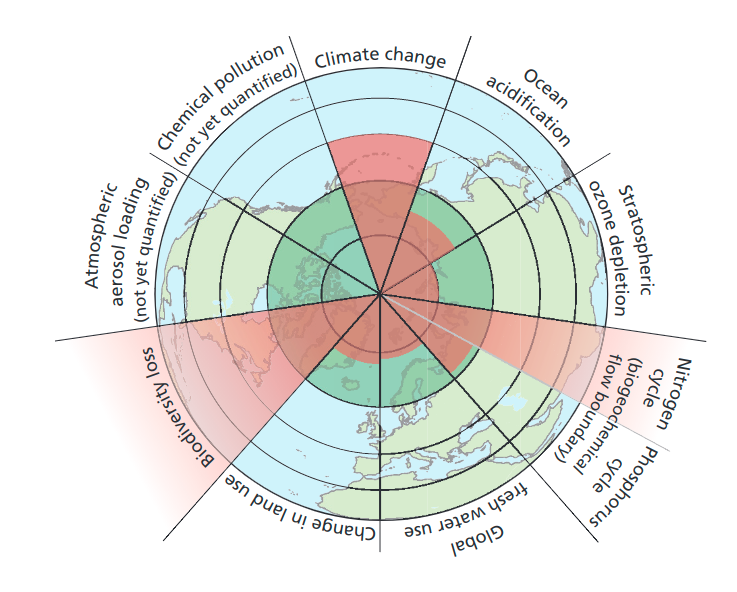
\includegraphics[scale=0.4]{Figures/chap2/Planetary_Boundaries.png}
	\caption[Planetary Boundaries]{Planetary Boundaries. From \cite{rockstromSafeOperatingSpace2009}}
	\label{fig:boundaries}
\end{figure}

Gini coefficient

Risks of business as usual



\begin{table}[h]
\begin{minipage}{\textwidth}

\caption[Estimated impacts of "business-as-usual" by domain and region.]{Estimated impacts of "business-as-usual" by domain and region. Adapated from \cite{rockstromSustainableDevelopmentPlanetary2013} and \cite{sachsAgeSustainableDevelopment2015} \protect\footnotemark[1]}
\label{table:bau}
\begin{center}
\tiny
\begin{tabular}{ | L{2cm} | C{1cm} | C{1cm} | C{1cm} | C{1cm} | C{1cm} | C{1cm} | C{1cm} | C{1cm} | } \hline
& North America & Latin America \& Caribbean & Europe & Middle East \& North Africa & Sub-Saharan Africa & South \& Central Asia & Southeast Asia \& Pacific & East Asia \\ \hline

Food Insecurity \& Malnutrition & & & & \cellcolor{red!25} H & \cellcolor{red!25} H & \cellcolor{red!25} H & \cellcolor{yellow!25} M  & \cellcolor{yellow!25} M \\ \hline

Poverty & & & & \cellcolor{yellow!25} M & \cellcolor{red!25} H & \cellcolor{red!25} H & \cellcolor{yellow!25} M  & \cellcolor{yellow!25} M  \\ \hline

Land Use Change & & \cellcolor{red!25} H & & & \cellcolor{red!25} H & \cellcolor{yellow!25} M  & \cellcolor{yellow!25} M  & \cellcolor{yellow!25} M  \\ \hline

Soil Degradation & & & & \cellcolor{yellow!25} M  & \cellcolor{red!25} H & \cellcolor{red!25} H   & \cellcolor{yellow!25} M  & \cellcolor{red!25} H   \\ \hline

Water Shortage & \cellcolor{yellow!25} M & & & \cellcolor{red!25} H & \cellcolor{red!25} H & \cellcolor{red!25} H & \cellcolor{yellow!25} M  & \cellcolor{yellow!25} M \\ \hline

Water \& Air Pollution & \cellcolor{yellow!25} M & & \cellcolor{yellow!25} M & \cellcolor{yellow!25} M  & &\cellcolor{red!25} H  & \cellcolor{red!25} H  & \cellcolor{red!25} H \\ \hline

Biodiversity Loss & \cellcolor{yellow!25}  & \cellcolor{red!25} H  & \cellcolor{yellow!25} M & \cellcolor{yellow!25} M  & \cellcolor{yellow!25} M & \cellcolor{yellow!25} M  & \cellcolor{red!25} H  & \cellcolor{red!25} H \\ \hline

Sea Level Rise & \cellcolor{yellow!25} M & \cellcolor{yellow!25} M & \cellcolor{red!25} H & \cellcolor{yellow!25} M & \cellcolor{red!25} H & \cellcolor{red!25} H &\cellcolor{red!25} H  & \cellcolor{red!25} H \\ \hline

Ocean Acidification &  \cellcolor{yellow!25} M & \cellcolor{red!25} H & \cellcolor{red!25} H & \cellcolor{yellow!25} M & \cellcolor{yellow!25} M  & \cellcolor{yellow!25} M & \cellcolor{red!25} H & \cellcolor{yellow!25} M \\ \hline
\end{tabular}
\end{center}
\end{minipage}
\end{table}

\footnotetext[1]{It should be noted that, despite the latter of these two sources citing the former, the two sources differ in noticeable ways, with no explanation provided in either document. Where they are in conflict, I have chosen to use the latter source. In the former source, there is also a error: Ocean Acidification in the Middle East / North Africa is listed as "H" but the cell is in yellow. The correct entry is not known, so I have gone with "M" in yellow here in order to avoid overstatement.}

\begin{figure}[h]
	\centering
	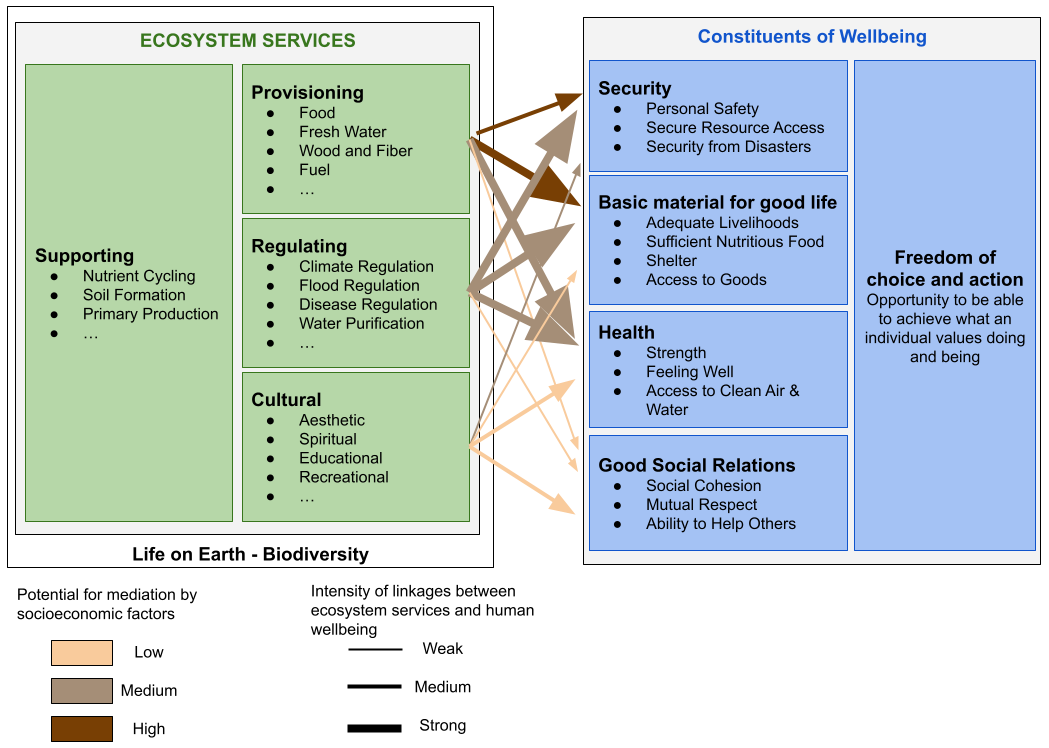
\includegraphics[scale=0.35]{Figures/chap2/services_wellbeing.png}
	\caption[Linkages between categories of ecosystem services and compotents of human wellbeing]{Linkages between categories of ecosystem services and compotents of human wellbeing. Adapted from \cite{reidEcosystemsHumanWellbeing2005}}
	\label{fig:services_wellbeing}
\end{figure}

Historically, surveys and quantifications of the natural environment focused primarily, or even entirely, on resources that could be extracted and exploited for economic benefit. In early forest surveys, for instance, "Missing... were all those parts of trees, even revenue-bearing trees, which might have been useful to the population but whose value could not be converted into fiscal receipts." \cite{scottSeeingStateHow2020}

\subsubsection{What about the Sustainable Development Goals?}


Jeffrey Sachs, "Our new era will son be described by new global goals, the \acp{sdg}. \cite{sachsAgeSustainableDevelopment2015}




Talk about \acp{mdg} and \acp{sdg}, pull from my previously written articles, also \cite{unitednationsWhoWillBe2013}




\subsection{Why Earth Observation Imagery}

This possibility was known even from the earliest days of remote observation. As Jennifer Light recorded, "one proponent [from the last 1940s] explained, photointerpretation data did not directly provide 'social data,' yet they were 'pertinent to social research needs in so far as such 'physical data' have meaningful sociological correlates." \cite{lightWarfareWelfareDefense2005} In the succeeding decades, the degree to which humans have altered the surface of our planet has only increased and, as a result, we can now also infer a great deal more about humans from images of that surface.

This was not always the case. For most of the early history of satellite observation, imagery was kept highly classified and zealously guarded, to the extent that Congressman George Brown Jr., who was integral in the establishment of the US \ac{ostp}, the \ac{epa}, and the \ac{ota}, resigned from his post in the House Intelligence Panel in protest over the enforced secrecy in even discussing the topic \cite{healyRepBrownQuits1987, barry1992mappings}

In the 1970s and early 1980s, Landsat data was a government-managed operation that provided products at a low-cost, based primarily on the cost of reproduction. In the 1980's, however, the program was transfered to a private entity and prices were increased by more than an order of magnitude and significant copyright restrictions were put in place. \cite{mchaffieManufacturingMetaphors1994}


By the early 1970's five rationales for using satellite imagery in city planing had become widespread \cite{lightWarfareWelfareDefense2005}:
\begin{enumerate}[itemsep=0pt,parsep=0pt]
	\item{It offers a synoptic, total view of the complex system in a given area.}
	\item{Satellites provide repetitive, longitudinal coverage.}
	\item{Satellite inventories were more efficient and up-to-date than ground surveys.}
	\item{Remote sensing was objective.}
	\item{Satellites produced digital imagery that could be easiliy combined with ground-based data in novel \acp{gis}.}
\end{enumerate}

Despite these rationales, cities and metropolitan areas largely elected not to use satellite imagery for several decades, choosing instead to rely on aerial imagery and ground-based surveys \cite{lightWarfareWelfareDefense2005}. The reasons for this are many, but probably include that many of these rationeles were overstated for their day. Insufficient resolution and inconsistent coverage limited intra-urban use. While satellite imagery provides a wonderful decades-long longitudinal dataset now, it did not at the time. Satellite imagery was still heavily dependent on human photointerpretation, undermining the argument that the data was "objective" in any meaningful sense. Finally the cost and specialization required to effectively use the data limited its ability to be combined with other datasets. Black-and-white aerial imagery provided sufficient resolution, oblique angles, and immediate interpretability to even the untrained eye. Plus cities were compact enough that the advantages of scale offered by satellites largely did not come into play. Ultimately, while \ac{gis} technology was readily adopted by cities, satellite imagery was not. \cite{lightWarfareWelfareDefense2005}.

NASA "did not go a long way toward incorporating remote sensing into day-to-day practices in city planning agencies. This was compounded by the fact that far more academics than local government officials participated in these experiments, providng applications of satellite data that were almost always a step removed from urban mangers' needs." \cite{lightWarfareWelfareDefense2005} [Talk about EVDT's efforts to fix this, plus that SERVIR suggests that maybe NASA has changed too.]

One of the first use of non-visual imagery for such applications was in 1970, when the city of Los Angeles used aerial infrared imagery to identify unsound housing, and, by 1972, had integrated this imagery with other datasets into a digital decision support system for assessing urban blight \cite{lightWarfareWelfareDefense2005}.

"The geography agenda is distorted by being data-led... The first law of geographical information: the poorer the country, the less and the worse the data." (\cite{overton1991further} as paraphrased by \cite{taylorGeographicInformationSystems1994}) 

\subsection{Why GIS and Decision Support?}

\ac{gis} originated in the 1960's and 70's with the Canda Geographic Information System and the US Bureau of the Census. \cite{goodchildGeographicInformationSystems1994}

"GIS allows geographers to integrate diverse types of data over different spatial scales from the regional to the global, while the advanced capabilities of GIS for organizing and displaying these data transofrm the geographer's view of the world." (\cite{tomlinsonPRESIDENTIALADDRESSGEOGRAPHIC1989} as paraphrased in \cite{vereginComputerInnovationAdoption1994})

One key moment in the development of \ac{gis} as we know it, was ESRI's creation of the shapefile format (which links geometries with data in a standardized, if somewhat limited, fashion) in the late 1980's, and, more importantly, their open publishing of the format, allowing others to create and manipulate such files \cite{goodchildModelingEarth2011}. 

As Maguire et al. wrote back in 2001, "It is not fanciful to suggest that by the end of the century \ac{gis} will be used every day by everyone in the developed world for routine operations." \cite{maguireGeographicalInformationSystems1991}

\ac{pgis}: Refer to macro-micro framework from Table 2.1, pg.17. What parts this thesis covers and what parts we envision EVDT covering in the long term. Also refer to EAST2 model on pg. 21 \cite{jankowskiGISGroupDecision2001}

\begin{table}[h]
\caption[Generic macro-micro, participtory decision strategy]{Generic macro-micro, participtory decision strategy. Adapted from \cite{jankowskiGISGroupDecision2001}}
\label{table:macro-micro}
\begin{center}
\begin{tabular}{ L{3cm} L{4cm}  L{4cm} L{4cm}} \hline
& \multicolumn{3}{c}{\textit{Macro-phases in a decision strategy}}  \\ \cline{2-4}

\textit{Micro-activities in a decision strategy} & \textbf{\textit{1. Intelligence}} about values, objectives, and criteria & \textbf{\textit{2. Design}} of a set of feasible options &  \textbf{\textit{3. Choice}} about recommendations \\ \hline

\textbf{A. Gather...} & issues to develop and refine \textbf{value trees} as a basis for objectives & \textbf{primary criteria} as a basis for option generation & \textbf{values, criteria, and option list scenarios} for an evaluation \\ \hline

\textbf{B. Organize...} & \textbf{objectives} as a basis for criteria and constraints & and apply approaches(es) for \textbf{option generation} & approaches to \textbf{priority and sensitivity analyses} \\ \hline

\textbf{C. Select...} & \textbf{criteria} to be used in analysis as a basis for generating options & the \textbf{feasible option list} & \textbf{recommendation} as a prioritized list of options \\ \hline

\textbf{D. Review...} & criteria, \textbf{resources, constraints,} and \textbf{standards} & \textbf{option set(s)} in line with resources, constraints, and standards & \textbf{recommendation(s)} in line with original \textbf{value(s), goal(s),} and \textbf{objectives} \\ \hline

\end{tabular}
\end{center}
\end{table}

\begin{figure}[h]
	\centering
	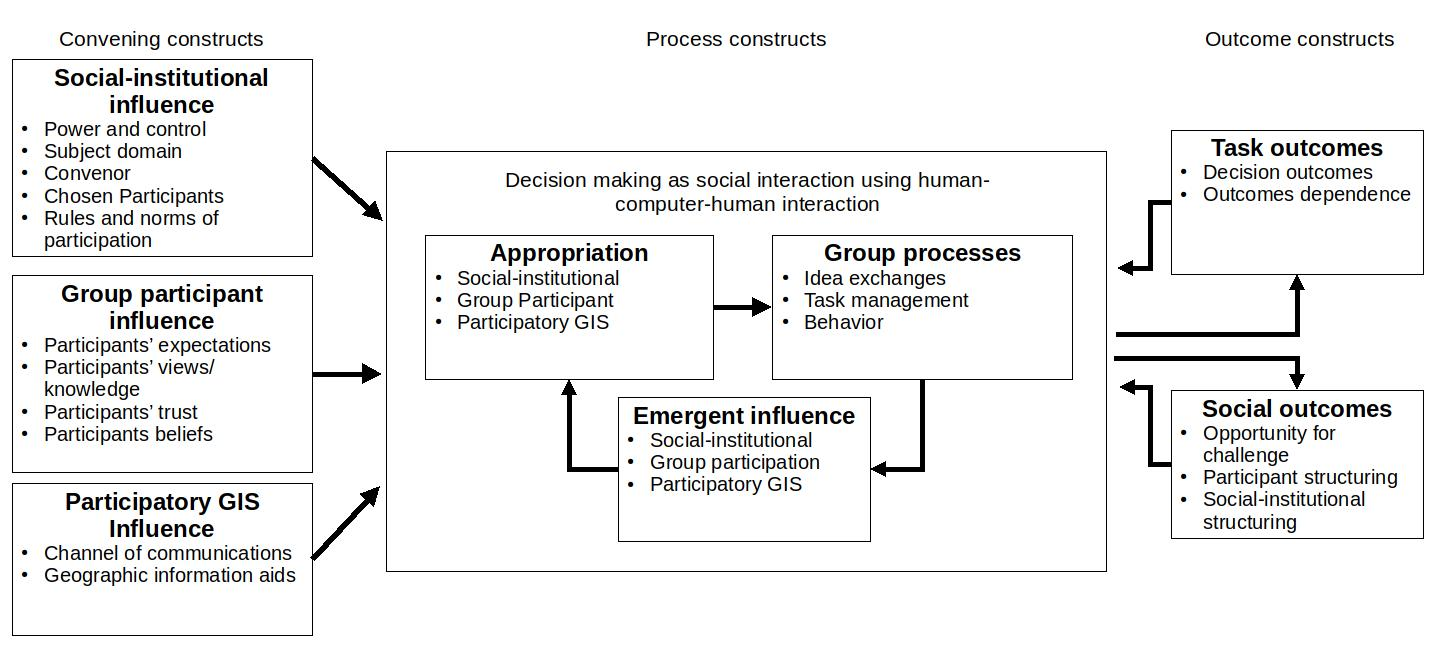
\includegraphics[scale=0.4]{Figures/chap2/east2.jpg}
	\caption[Enhanced Adaptive Structuration Theory 2 (EAST2)]{Enhanced Adaptive Structuration Theory 2 (EAST2). Adapted from \cite{jankowskiGISGroupDecision2001}}
	\label{fig:east2}
\end{figure}


Jankowski and Nyerges lay out seven common design requirements for spatial decision support tools \cite{jankowskiGISGroupDecision2001}:

\begin{enumerate}
    \setlength{\itemsep}{0pt}%
    \setlength{\parskip}{0pt}%
	\item{A spatial decision support system for collaborative work should offer decisional guidance to users in the form of an agenda.}
	\item{A system should not be restrictive, allowing the users to select tools and procedures in any order.}
	\item{A system should be comprehensive within the realm of spatial decision problems, and thus offer a number of decision space exploration tools and evaluation techniques.}
	\item{The user interface should be both process-oriented and data-oriented to allow an equally easy access to task-solving techniques, as well as maps and data visualization tools.}
	\item{A system should be capable of supporting facilitated meetings and hence, allow for the information exchange to proceed among group members, and between group members and the facilitator. It should also allow space- and time-distributed collaborative work by facilitating information exchange, electronic submission of solution options, and voting through the internet.}
	\item{A system functionality should include extensive multiple criteria evaluation capabilities, sensitivity analysis, specialized maps to support the enumeration of preferences and comparison of alternative performance, voting, and consensus building tools.}
	\item{A system should provide ncessary functionality to support needs of an advanced user without overwhelming a novice who needs a user-guiding interface.}
\end{enumerate}



\begin{figure}[h]
	\centering
	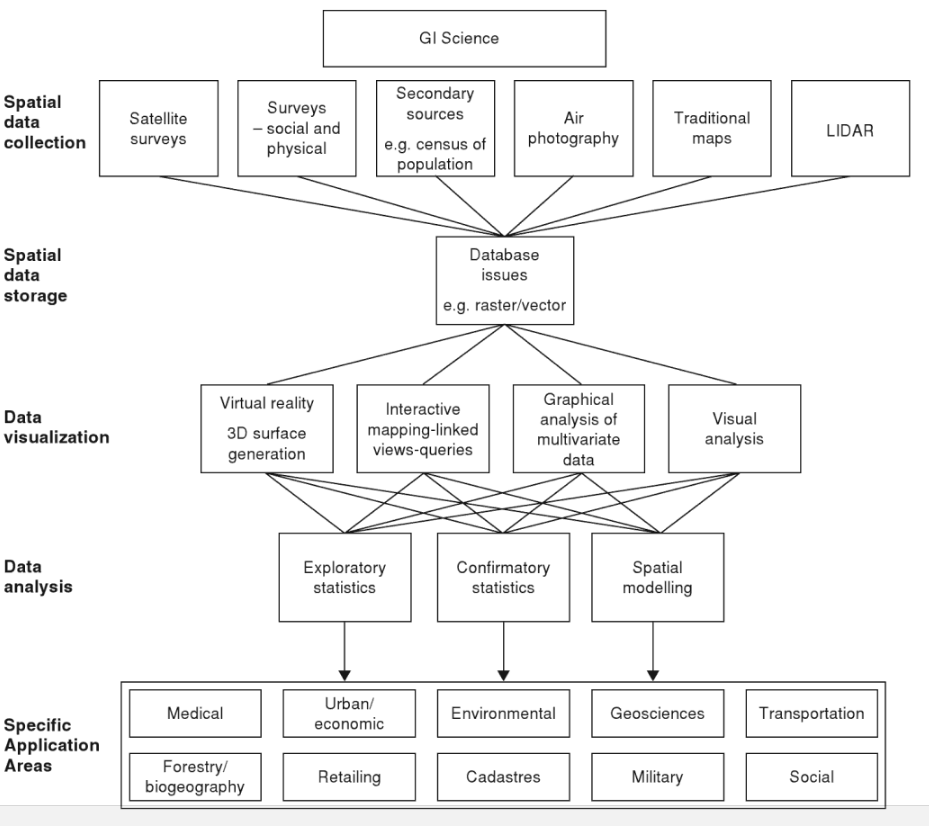
\includegraphics[scale=0.4]{Figures/chap2/GIScience.png}
	\caption[Overview of Geographical Information Science]{Overview of Geographical Information Science. From \cite{fotheringhamGeographicInformationScience2007}}
	\label{fig:giscience}
\end{figure}

\begin{figure}[h]
	\centering
	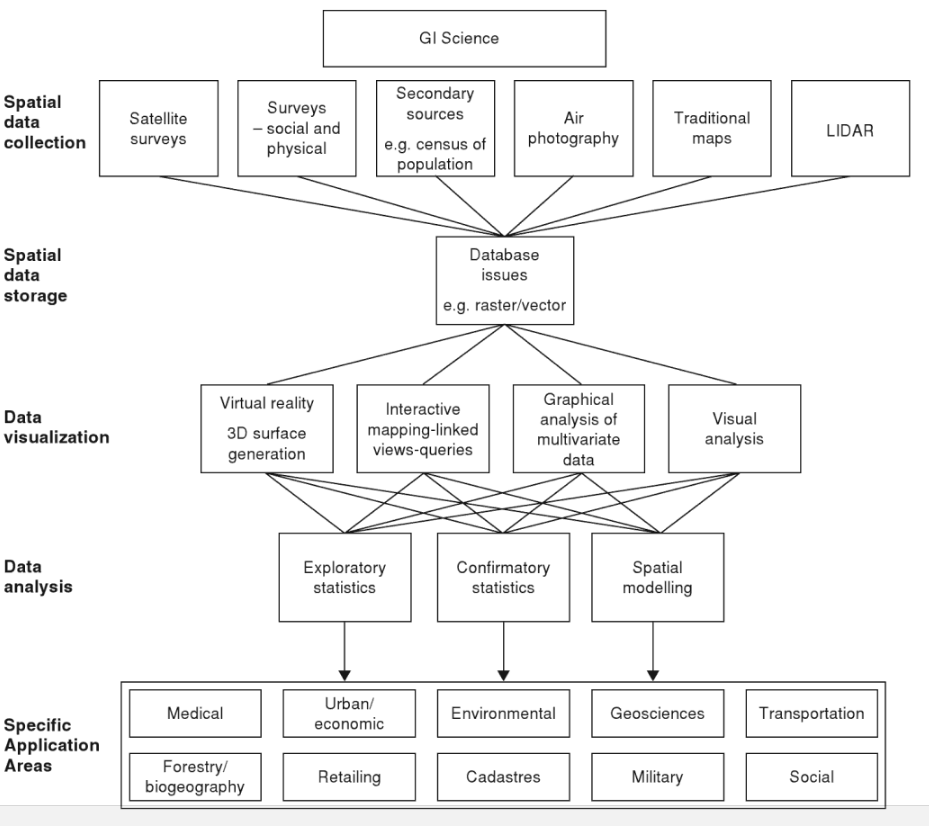
\includegraphics[scale=0.4]{Figures/chap2/GIScience.png}
	\caption[The marketplace for geographic data]{The marketplace for geographic data. From \cite{cowenAvailabilityGeographicData2007}}
	\label{fig:marketplace}
\end{figure}


the meeting arrangment that EVDT supports, \ref{table:meeting_arrangements}

\begin{table}[h]
\caption[Different types of meeting arrangements]{Different types of meeting arrangements. Adapted from \cite{jankowskiGISGroupDecision2001}}
\label{table:meeting_arrangements}
\begin{center}
\begin{tabular}{ L{3cm} L{5.5cm}  L{5.5cm}}  \hline
 & \textit{Same time} &\textit{Different time}  \\ \cline{2-3}
\textbf{\textit{Same place}} & \textbf{Conventional Meeting} \qquad \textit{Advantage:} 
\vspace{-5mm}
\begin{itemize}
    \setlength{\itemsep}{0pt}%
    \setlength{\parskip}{0pt}%
	\item{face-to-face expressions}
	\item{immediate response}
\end{itemize} &
\textbf{Storyboard meeting} \qquad \textit{Advantage:} 
\vspace{-5mm}
\begin{itemize}
    \setlength{\itemsep}{0pt}%
    \setlength{\parskip}{0pt}%
	\item{scheduling is easy}
	\item{respond anytime}
	\item{leave-behind note}
\end{itemize} 
\\
& \textit{Disadvantage:} 
\vspace{-5mm}
\begin{itemize}
    \setlength{\itemsep}{0pt}%
    \setlength{\parskip}{0pt}%
	\item{scheduling is difficult}
\end{itemize} &
\textit{Disadvantage:} 
\vspace{-5mm}
\begin{itemize}
    \setlength{\itemsep}{0pt}%
    \setlength{\parskip}{0pt}%
	\item{meeting takes longer}
	\item{difficult to maintain in the long run}
\end{itemize} 
\\ \hline

\textbf{\textit{Different place}} & \textbf{Conference call meeting} \qquad \textit{Advantage:} 
\vspace{-5mm}
\begin{itemize}
    \setlength{\itemsep}{0pt}%
    \setlength{\parskip}{0pt}%
	\item{no need to travel}
	\item{immediate response}
\end{itemize} &
\textbf{Distributed meeting} \qquad \textit{Advantage:} 
\vspace{-5mm}
\begin{itemize}
    \setlength{\itemsep}{0pt}%
    \setlength{\parskip}{0pt}%
	\item{scheduling is convenient}
	\item{no need to travel}
	\item{submit response anytime}
\end{itemize} 
\\
& \textit{Disadvantage:} 
\vspace{-5mm}
\begin{itemize}
    \setlength{\itemsep}{0pt}%
    \setlength{\parskip}{0pt}%
	\item{limited personal perspective from participants}
	\item{meeting protocols are difficult to interpret}
	\item{difficult to maintain meeting dynamics}
\end{itemize} &
\textit{Disadvantage:} 
\vspace{-5mm}
\begin{itemize}
    \setlength{\itemsep}{0pt}%
    \setlength{\parskip}{0pt}%
	\item{meeting takes longer}
	\item{meeting dynamics are different from normal meeting ("netiquette" instead of face-to-face etiquette)}
\end{itemize} 
\\ \hline
\end{tabular}
\end{center}
\end{table}

Levels of decision support \cite{jankowskiGISGroupDecision2001}:

\begin{enumerate}[itemsep=0pt,parsep=0pt]
	\item{\textit{Basic information handling support}}
%	\vspace{-5mm}
		\begin{enumerate}[itemsep=0pt,parsep=0pt,topsep=0pt, partopsep=0pt]
			\item{Information management}
			\item{Visual aids}
			\item{Group collaboration support}
		\end{enumerate}
%	\vspace{-5mm}
	\item{\textit{Decision Analysis Support}}
%	\vspace{-5mm}
		\begin{enumerate}[itemsep=0pt,parsep=0pt,topsep=0pt, partopsep=0pt]
			\item{Option modeling}
			\item{Choice models}
			\item{Structured group process techniques}
		\end{enumerate}
%	\vspace{-5mm}
	\item{\textit{Group reasoning support}}
%	\vspace{-5mm}
		\begin{enumerate}[itemsep=0pt,parsep=0pt,topsep=0pt, partopsep=0pt]
			\item{Judgement refinement/amplification techniques}
			\item{Analytical reasoning methods}
		\end{enumerate}
\end{enumerate}

EVDT is partially based on Tomlin's cartographic modeling concept from 1990. "The cartographic modleing approach attemps to generalize and standardize the analytic and synthetic capabilities of geopgrahical information systems. It does so by decomposing data, data-processing tasks, and data-rpocessing control notation into elementary components that can be recomposed with relative ease and great flexibility." \cite{tomlinGISCartographicModeling2012}

"Scenario planning is a method of long-term strategic planning that creates representations of multiple, plausible futures of the system of interest." It arose in military and corporate strategies \cite{goodspeedScenarioPlanningCities2020} 

[Refer to my old RAND citations about scenario planning]

"A scenario-based strategic plan is... appropriate for vision, framework, comprehensive, system, and redevelopment plans and for those with long time horizons and low or moderate detail." \cite{goodspeedScenarioPlanningCities2020} 

\textit{Oregon Scenario Planning Guidelines} proposes a six-step process for scenario planning ( \cite{oregonsustainabletransportationinitiativeScenarioPlanningGuidelines2017} as paraphrased by \cite{goodspeedScenarioPlanningCities2020}:

\begin{enumerate}[itemsep=0pt,parsep=0pt]
	\item{Create a framework for the scenario planning process.}
	\item{Select evaluation criteria.}
	\item{Set up for scenario planning: evaluation tools ,data, and building blocks.}
	\item{Develop and evaluate base-year conditions and reference case.}
	\item{Develop and evaluate alternative scenarios}
	\item{Select the preferred scenario}
\end{enumerate}

Goodman describes four primary kinds of planning support models \cite{goodspeedScenarioPlanningCities2020}: 

\begin{enumerate}[itemsep=0pt,parsep=0pt]
	\item{Generic Systems Models: Developing a typically non-spatial abstract representation of a system and analyzing how it functions. System dynamics is a classic example.}
	\item{Economic and Demographic Models: The set of techniques that focus on changes in employment of particular sectors and in populuation of different characteristics. Klosterman is the classic text on these methods. \cite{klostermanCommunityAnalysisPlanning1990}}
	\item{Place-Type Development and Analysis: Tools used to simulate future outcomes based on land use, zoning, population density, etc. CommunityViz is an example of this \cite{walkerPlannersGuideCommunityViz2017}.}
	\item{Urban Systems Models: Essentially a combination of generic systems modeling and place-type development and analysis models to accurately represent spatial phenomena over time, such as transportation networks and organic growth. Examples include cellular automata and spatial interaction models.}
\end{enumerate}

The city of Chicago has developed \ac{gis} apps to visualize food deserts and develop maps of where new supermarkets are both needed and economically vialbe. \cite{goldsmithResponsiveCityEngaging2014} 

"Non-human animals are rarely considered within the realms of social theory, and yet... animals can be regarded as a 'marginal social group' that is 'subjected to all manner of socio-spatial inclusions and exclusions.'" (\cite{philolAnimalsGeographyCity1995,westcoatBringingAnimalsBack1995,wolchAnimalGeographiesPlace1998}as paraphrased in \cite{harrisRethinkingMapsMorethanhuman2011}) I would argue that plants, particularly non-domesticated plants, could similarly be regarded as a marginal social group that is often neglected by decision support tools.

The motivation for combining so many variables from different disciplines stems from both push and pull factors. The push factors are the simple increase in availability of data, as has already been described, along with the increase in the interoperability of the variables (which the work described in this thesis is trying to help contribute to). The primary pull factor is our increased understanding of - and appreciation for - the complex relationships between these domains, relationships that were previously ignored in analyses \cite{gaheganMultivariateGeovisualization2007}. 

\subsection{Why Collaborative and Open Source?}

"It is the geomorphologist who is best able to choose the dta model for representation of terrain in a GIS, not the computer scientist or the statistician, and it is the urban geographer who is best able to advicse on how to represent the many facets of hte urban environment in a GIS designed for urban planning." \cite{goodchildGeographicInformationSystems1994}

"Knowing \textit{how} refers to the ability to do something...Knowing \textit{that} refers to knowledge about how something works." \cite{curryGeographicalInformationSystems1994} Vida seeks to help people move from how to that through collaboration and open source. 

In 1994, McHaffie wrote that "for billiions the possibility of accessing the best technolog yand information made available through digital communications network will always be a luxury. Cartographic information, digital or otherwise, becomes a commodity in its mass production and marketing." \cite{mchaffieManufacturingMetaphors1994}

"It is impossible to have sustainable and equitable development without free access to reliable and accurate information." \cite{benmouffokInformationDecisionMaking1993}

"Without equitable access to GIS data and technology, small users, local governments, nonprofit community agencies, and nonmainsream groups are significantly disadvantaged in their capacity to engage in the decision-making process." (\cite{edney1991strategies} as paraphrased in \cite{harrisPursuingSocialGoals1994})

Participatory \ac{gis} has been successfully used in South Africa to try and overcome such issues of inequal access and use of \ac{gis} technology. They sought to achieve five specific objectives \cite{harrisPursuingSocialGoals1994}: 

\begin{enumerate}[itemsep=0pt,parsep=0pt]
	\item{Enhanced community/development planner interaction in a research and policy agenda setting}
	\item{The integration of local knowledge with exogenous technical expertise.}
	\item{The spatial representation of relevant aspects of local knoweledge.}
	\item{Genuine community access to, and use of, advanced technology for rural land reform.}
	\item{The education of "expert" rural land use planners about the importane of popular participation in policy formulation and implementation.}
\end{enumerate}

Expansion of choice is valuable for both intrinsic (for its own sake) and instrumental (to attain preferred positions) reasons \cite{senFreedomChoiceConcept1988}. \ac{evdt} primarily addresses the latter reason, by allowing for more selecting a preferred choice that might otherwise have been overlooked.

Giles Deleuze on Michel Foucault: "You have taught us something absolutely fundamental: The indignity of speaking on someone else's behalf" \cite{sheridanMichelFoucaultWill2003}


While collaborations certainly can introduce additional difficulties, including cultural conflicts and issues of interpersonal trust, they are also immensely rewarding \cite{tullochInstitutionalGeographicInformation2007}.

While \ac{ppgis} refers to involving the public in both the creation and the use of data, in practice, it has tended to focus primarily on the former, thus situating it as a form of \ac{gisc} rather than application \cite{weinerParticipatoryGeographicInformation2007}. For example, in Washington state in 2002 , several American Indian tribes were using \ac{gis} technology to "inventory, analyze, map, and make descisions regarding tribal resources... includ[ing] timber production, grazing and farm land, water rights, wildlife, native plants, cultural sites, environmental data and hazardous site monitoring, historical preservation, health and human resources." \cite{bondCherokeeNationTribal2002}

Digital tools that provide open data (1) frees data from bureaucractic constraints, allowing real time combination of data from different souces; (2) construct a loop between government and the community in which cooperation builds respect continuously; (3) Enable two-way communication, promotiving collaboration \cite{goldsmithResponsiveCityEngaging2014}.

"The open source movement at its core stands for the development of source code... in a completely open and free way. Pragmatically, this manifests itself as a methodology of making code freely available to anyone who may wish to access it for any purpose, unconditionally. Concurrently, open source is for many a philosophical approach to software development, and is see as the only truly sustainable approach to software development... In both its execution as a model for making possible new forms of collaborative work, and its philosophical underpinnings of sustainability and openness, it is an essential component in and fluence upon a computer-based mapping solution." \cite{williamsonTheirworkDevelopmentSustainable2011}

"Map studies needs to open the 'black boxes' of mapping software, to start to interrogate algorithms and databases, and in particular to investigate the production of ready-made maps that appear almost magically on the interfaces of gadgets and devices we carry and use everyday, often without much overt thought about how they work and whose map they project onto their interface." \cite{dodgeMappingModesMethods2011}


\subsection{Why Systems Engineering?}

Refer to Crawley, deWeck, de Neufville, Rhodes, my earlier papers, etc.

"Sustainable development is also a science of complex systems" \cite{sachsAgeSustainableDevelopment2015}

"Sustainable Development involves not just one but four complex interacting systems. It deals with a global economy...; it focuses on social interactions...; it analyzes the changes in complex Earth systems...; and it sutdies the problems of governance." \cite{sachsAgeSustainableDevelopment2015} [Compare this to the EVDT framework]

The growth and development of cities is a complex system. Much work has been done using cellular automata and fractals to model them \cite{battyCitiesComplexity2005}

Urban planners have been seeking to develop useful indices and indicators akin to those used in engineering and remote observation contexts for decades (Section 1, Cahpter 3 of \cite{boyceFrameworkDefiningApplying1972}


"Futures planning as described and prescribed by futurists is different from planning \textit{for} te future; it is an attempt to manipulate or plan \textit{the} future. A basic characteristic of this orientation is the use of such terms as "designing," "inventing," or even "making" the future. When the future is being planned for, rather than designed, the implication is that the planner is trying to make specific and limited accomodations to the broad and overall characteristics of the future he considers either immutable or too formidable to be fundamentally rearranged or restructured." \cite{robinsonDecisionmakingUrbanPlanning1972}

"If alternatives are not carefully related to goals and objectives there is the real danger that they will either fail to reflect certain important issues which the planning process to being used to study, or worse still, be almost irrelevant... Alternatives must reflect the goals sought; the means must reflect the ends." \cite{mcloughlinChartingPossibleCourses1972}



Position \ac{evdt} using the different dimensions of models proposed in \cite{harrisQuantitativeModelsUrban1972}:


Sachs argues that two specific tools are important for implementing the \acp{sdg}: backcasting and technology road-mapping \cite{sachsAgeSustainableDevelopment2015}. Systems engineering is well equiped to address both of these.

\begin{enumerate}[itemsep=0pt,parsep=0pt]
	\item{descriptive vs. analytic}
	\item{holistic vs. partial}
	\item{macro vs. micro}
	\item{static vs. dynamic}
	\item{deterministic vs. probabilistic}
	\item{simultaneous vs. sequential (directly calculate the output or go through intermediate phases)}
\end{enumerate}


In order for cost-benefit analysis to maximize economic welfare, the following conditions must be met \cite{krutillaWelfareAspectsBenefitCost1961}:

\begin{enumerate}[itemsep=0pt,parsep=0pt]
	\item{Opportunity costs are borne by beneficiaries in  such wise as to retain the initial income distribution}
	\item{The initial income distribution is in some sense "best}
	\item{The marginal social rates of transformation between any two commodities are everywhere equal to their corresponding rates of substitution except for the area(s) justifying the intervention in question}
\end{enumerate}

More details modeling, as well as breaking down specific costs and benefits (as opposed to converting them to monetary terms and summing them) and attributing them to specific goals, can circumvent these constraints, though at the cost of increased complexity \cite{hillGoalsAchievementMatrixEvaluating1972}.

This work does not directly incorporate mechanisms for multi-stakeholder negotiation or tradespace exploration, but it is amenable to extension with such mechanisms (refer to SEAri research)

The Law of requisite variety from the field of cybernetics says that the variety (the number of elements or states) of the control device must be at least equal to that of the disturbances \cite{ashbyRequisiteVarietyIts1991}. Any development plan is going to fall far short of the variety expressed by human society and the natural environment. Planning efforts must then make reliance on the natural homeostasis behavior of such systems and of more flexible, ad hoc measures not specified in the plan in order to make up the difference in variety. \cite{mcloughlinSystemGuidanceControl1972}

Refer to epoch-era analysis and tie that in to scenario planning history.

Goodchild defines six different \ac{gis} data field model types and states that "no current \ac{gis} gives its users full access to all six":

\begin{enumerate}
    \setlength{\itemsep}{0pt}%
    \setlength{\parskip}{0pt}%
	\item{Sample randomly located points (e.g. weather stations, \ac{lidar} data)}
	\item{Sample randomly from a grid of regularly space points (e.g. many data validation studies}
	\item{Divide the area into a grid in which each rectangular cell records the average, total, or dominant value; i.e. raster data (e.g. satellite imagery)}
	\item{Divide the area into homogenous regions and record the average, total, or dominant value in each area (e.g. census data, soil maps)}
	\item{Record the locations of lines of fixed values (e.g. contour or isopleth maps}
	\item{Divide the area into irregular shaped triangles and assume the field varies linearly within each (e.g. some \acp{dem})}
\end{enumerate}

In the mid 90's, \ac{GIS} had several limitations \cite{goodchildGeographicInformationSystems1994}:

\begin{itemize}
    \setlength{\itemsep}{0pt}%
    \setlength{\parskip}{0pt}%
	\item{Two-dimensional, with some excursions into three}
	\item{Static, with some limited support for time dependence}
	\item{Limited capabilities for representing forms of interaction between objects}
	\item{A diverse and confusing set of data models}
	\item{Dominated by the map metaphor}
\end{itemize}

\section{EVDT Framework}

Is not itself a means of planning and implementing projects. It is not a full life-cycle tool such as \ac{ppbs} \cite{hatryCriteriaEvaluationPlanning1972}

\section{Intended Use Cases / Applications}

While \ac{evdt} does not include any concrete spatial scale requirements, it is often the most straightforward to apply to it at a a relatively local scale, like much of the early history of \ac{gis} applications \cite{tullochInstitutionalGeographicInformation2007}. Most of the applications to date have been at the area of a metropolitan area or that of a small province.


Commonly has to do with \acp{cpr}. Talk about the three common ways of managing \acp{cpr}: Central management, privatization, self-management. Bring in Table \ref{table:cpr_design}  showing design principles of long-enduring self-management institutions. Refer to successful aspects of the water basin in California (incremental and sequential process to reduce the costs of local institutional supply, shared information at each step, intermediate benefits from initial investments were realized prior to larger investments, transformed structure of incentives within which fuure strategic decisions can be made) (pg. 137. \cite{ostromGoverningCommonsEvolution2015}

\begin{table}[h]
\caption[Design principles illustrated by long-lasting CPR institutions]{Design principles illustrated by long-lasting \ac{cpr} institutions. Adapted from \cite{ostromGoverningCommonsEvolution2015}}
\label{table:cpr_design}
\begin{center}
\begin{tabular}{ L{0.5cm} L{8cm}} \hline
1. & Clearly defined boundaries \\
2. & Congruence between appropriation and provision rules and local conditions \\
3. & Collective-choice arrangements \\
4. & Monitoring \\
5. & Graduated sanctions \\
6. & Conflict-resolution mechanisms \\
7. & Minimal recognition of rights to organize \\
\multicolumn{2}{l}{\textit{For CPRs that are parts of larger systems:}} \\
8. & Nested enterprises \\ \hline
\end{tabular}
\end{center}
\end{table}

We also 

Harris et al. have pointed out that reliance on mapping products to designate certain geographic areas for conservation has several negative consequences, including: 

\begin{itemize}
    \setlength{\itemsep}{0pt}%
    \setlength{\parskip}{0pt}%
	\item{solidifying a notion that humans and non-human others are, and should be, separate.}
	\item{privileging those voices and perspectives that have access and expertise related to Western cartographic approaches and GIScience in conservation debates.}
	\item{favoring those spaces, ecosystems, and natures that may be "more mappable" for protection over other areas.}
	\item{cementing an overly-limited territorial approach to conservation, in ways that potentially sideline non-territorial approaches.}
	\item{consolidating an overly-fixed and static approach to sonservation, rather than enabling approaches that may be more seasonal, fluid, or appropriate for shifting and evolving ecological conditions and needs.}
\end{itemize}

\section{Critiques}

\begin{itemize} \setlength{\itemsep}{0pt} \setlength{\parskip}{0pt} 
	\item{Systems engineering is an inherently elitist methodology whose primary use is to defend the oppressive status quo and eke out greater "efficiencies" with little regard for societal consequences.}
	\item{Western-run technocratic planning and international development perpetuates colonialism, typically fails in its own goals, and merely destroys traditional communities.}
	\item{Sustainable development, as it is commonly used, is essentially meaningless and the \acp{sdg} are likewise such a potpourri of targets and indicators that they have little influence on what would have happened anyways.}
	\item{The effectiveness of scenario planning and most other forms of decision support is ambiguous at best, despite their long history. Another research project in this vein is thus fundamentally flawed and is not real science.}
	\item{Technology itself is at best a major contributor, if not the source of most of the problems you seek to address If you truly want to save the Earth and stop oppression, you should abandon technology rather than doubling down on it.}
\end{itemize}



\subsection{Technology is Bad}

"Keynes's point is that technology is crucial for the long haul of economic development." \cite{sachsAgeSustainableDevelopment2015}

"This slow rate of progress, or lack of progress, was due to two reasons - to the remarkable absence of important technical improvements and to the failure of capital to accumulate." [Cite Keynes 1930, page 2, as seen on page 74 of Sachs]

"Choosing the right technologies, we can achieve continued economic growth and also honor the planetary boundaries." \cite{sachsAgeSustainableDevelopment2015}

"Planning theorists have toooften accepted Habermas's view that technology is primarily associated with technical rather than moral rationality, which leads them to overlook technology's potential normative dimension... Even choosing a digital tool requires making value-laden judgements about what issues matter enough to be analyzed. Becaues digital tools typically inherit the worldviews and assumptions of their creators, even well-meaning applications of them can inhibit potentially valuable new ideas or critical perspectives." Goodspeed proposes the term \textit{tool of inquiry} to "describe the ideal in which tools are continually shaped, used, and tested by public users. \cite{goodspeedScenarioPlanningCities2020}

Passage by John Pickles \cite{picklesGroundTruthSocial1994}:

\blockquote{The Western trop of a public space in which people (usually "men") of good faith join in debate about their future, appropriated by industrial and urban forms of modernity as a mythic image of a democratic culture of debate and negotiation predicated on individual autonomy, private property, and state power has more recently been further appropriated by the news and communication media through their claim to be the embodiment of the modern civic arena. This trope of public space is now being reappropriated by the electronic age as its wish image - the promise and possibility of "information." The putative openness of new electronic information media and the rhetoric of "voice," "openness," and "information" - the trope of reasoned, open, uncoerced discourse in a public place - is appropriated to the project of social development and private profit.

But, like all highways, the information highway requires points of access, capital investment, navigation skills, and spatial and cultural proximity for effective use. Like the automobile highway, the information highway fosters new rounds of creative destruction and differentiates among users and between users and nonusers. It brings regions of diference under a common logic and technology, and throuhg differential access and use exacerbates old and crates new patterns of social and economic differentiation. While for some, information means the provision of alternatives and the satisfication of choice (even if a "choice" signifies a socially constructed yet now naturalized whim of the wealthy consumer), for others this postindustrialism (and its attendant postmodern cultural forms) must still be seen in the context of a political economy of graft, monopolism, and uneven dvelopment.

Such processes of territorial coonizations, globalization, and production of new scales of actoin contrast sharply with a technocultural ideology of enhanced autonomy and self-actualization, and severly complicates the assessment of hte rleationship between technological innovation and social change.}

Passage by Penley and Ross \cite{penleyTechnoculture1991}:

\blockquote{Wary, on the one hand, of the disempowering habit of demonizing technology as a satanic mill of domination, and weary, on the other, of the postmodernist celebrations of the technological sublime, we selected contributors whose critical knowledge might help provide a realistic assessment of the politics - the dangers \textit{and} the possibilities - that are currently at stake in those cultural practices touched by advanced technology.}

"GIS and informatics do open virtual space of 'real' social interaction, new communities of dialogue, and new interactive settings... Systems of informatics provide a potential source of counterhegemonic social action, and GIS... offers a diverse array of practical possibilities... Informatics are seen as a potential liberator of socially and politically marginalized groups, and thus a source of democratizing power for these newly networked groups." \cite{picklesRepresentationsElectronicAge1994}

I align myself with those who feel that "Even though the funding or research and development... of GIS and other imaging systems has come primarily from business, state, and military sources, advocates of the progressive potential information and imaging technologies argue that access is hard to deny, networks are difficult to control, information is readily accessible and used by individuals and groups with limited budgets and expertise, and the ability to use the technology in depth permits groups like environmental organizations to counter claims by polluters about their environmental impacts, by developers about likely local effects of runoff and ground water, and so on... GIS enables communities to make better decisions by providing access to more and better information. It offers more powerful tools for local planning agenceisl if offers exciting possibilities for data coordination, access, and exchange; and it permits more efficient allocation of resources, and a more open rational decision-making process." \cite{picklesRepresentationsElectronicAge1994} [maybe add a caveat talking about "rational"]

As pointed out by Pickles, historically within the GIS research community and its predecessors, there has been a certain "technocratic myopia" and unwillingness to consider novel, insurgent uses of GIS that has led critics to label it as an "inherently conservative form of analysis." \cite{picklesRepresentationsElectronicAge1994}

It was only in the late 1980's did scholars, informed primarily by Michel Foucault and Karl Marx, start challenging the idea that "cartography produces maps of truth in an objective, neutral, scientific fashion." \cite{kitchinThinkingMaps2011}

Cite Langdon Winner somewhere in here

"Mappings do not represent geographics of ideas; rather they effect actualization... Maps remake 'territory over and over again, each time with new and diverse consequences.'" (\cite{cornerAgencyMappingSpeculation1999} as paraphrased by \cite{kitchinThinkingMaps2011}

In some ways, we want to avoid making a seemless tool, as "the most significant impacts of technology tend to occur when the technology becomes indistringuishable from the fabric of every day life" (\cite{weinerComputer21stCentury1991} as paraphrased in \cite{vereginComputerInnovationAdoption1994}). This is not, unfortunately, not sufficient. "We all tend to defer to machines, which can seem more neutral, more objective" even when they are actively warning us of their limitations and fallibility \cite{eubanksAutomatingInequalityHow2018}.

Even the most ardent supporters of digital tools and data collection often fall into a sort of technological determinism. Stephen Goldsmith and Susan Crawford, who did a great deal to implement such technologies in New York City and Indianapolis, wrote that "the process of collection is not going to stop. We think, it fact, that it would be shortsighted and probably impossible to halt this natural evolution. That is all the more reason, then, to carefully establish policies covering data access, data security, and transparency with respect to its collections." \cite{goldsmithResponsiveCityEngaging2014}

"It is also not clear that geography's diversity is a flaw instead of a great strength. Geography is inherently eclectic because the discipline is defined only by a perspective on the world. However, those who advocate the computer as a means to unify geography have a particular conception of the discipline in mind, an empirical and pragmatic one that is by no means universally accepted." \cite{vereginComputerInnovationAdoption1994}

National mapping in the US originated in motives that were explicity of means of resource exploitation and control. \cite{mchaffieManufacturingMetaphors1994}

"Perhaps the 'frightened Africans' who once 'threw spears at an Aero Service aircraft' or the 'suspicious moonshiners in Appalachia' who 'took a few rifle shots' at aerial mappers did so not because the intentions of the mappers were 'not always understood,' but because those intenions, and the powerful forces being them, were understood only too well." \cite{mchaffieManufacturingMetaphors1994}

Cite the million dollar blocks \cite{kurganCloseDistanceMapping2013}, redlining visualizations, etc.

Smithsonian curator Lucy Fellowes: "Every map is someone's way of getting you to look at the world his or her way." \cite{henriksonPowerPoliticsMaps1994} We think EVDT is a means of getting people to think about sustainable development about antiracism, etc. 

For a clear example of a technologically produced geographic object having enormous postive impact, we can look no further than NASA's famous Blue Marble image, which, while perhaps more iconic than cartographic, is still undeniably a geospatial object, a map even, that has essentially created both "one-world" discourse and "whole-earth" discourse \cite{propenCartographicRepresentationConstruction2011},  

Similarly, the Sierra Club has made significant use of Google Earth in their efforts to garner support for conservation efforts in the US Arctic National Wildlife Refuge and elsewhere \cite{propenCartographicRepresentationConstruction2011}. 

As Krygier and Wood so playfully illustrated, maps are, fundamentally, propositions about that world that are asserting a fact and promoting an action. Because of this "you must accept responsibility for the realities you create with maps." \cite{krygierCeEstPas2011}

"The very notion that technologies are neutral must be directly challenged as a misnomer." \cite{nobleAlgorithmsOppressionHow2018}

"Design is purposeful in that it forges both pathways and boundaries in its instrumental and cultural use." (\cite{paceyCultureTechnology1983} as paraphrased in \cite{nobleAlgorithmsOppressionHow2018})

"Those who have hte power to design systems - classification or technical - hold the ability to prioritize hierarchical schemes that privilege certain tyeps of information over others." \cite{nobleAlgorithmsOppressionHow2018}

\subsection{Scenario Planning and Decision-Support is unfounded}


Often, however, so-called "strategic planning" is anything but. "A strategic plan might more closely resemble a project plan, with long lists of specific proposals and policies... many have relatively short time frames. Scenario planning may not make sense for these plans." \cite{goodspeedScenarioPlanningCities2020}

Many projections have been bad

\begin{figure}[h]
	\centering
	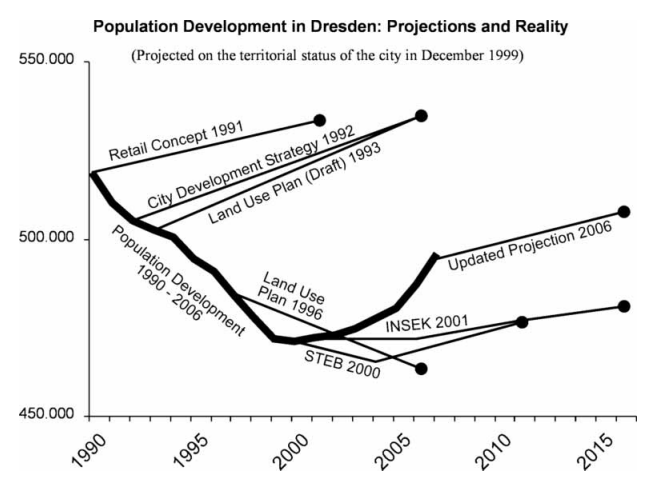
\includegraphics[scale=0.35]{Figures/chap2/dresden_projections.png}
	\caption[Population changes in Dresden compared to various projections]{Population changes in Dresden compared to various projections. From \cite{wiechmannErrorsExpectedAligning2008}}
	\label{fig:dresden_population}
\end{figure}


While forecasting can be problematic as it constitutes "someone else's understanding and judgement crystallized in a figure that then becomes a substitute for thinking," scenario planning instead allows users to "develop their own feel for the nature of the system, the forces at work within it, the uncertanties that underlies the laternative scenarios, and the concepts useful for interpreting key data." \cite{wackScenariosShootingRapids1985}

The evidence for such practices as scenario planning is decidedly mixed. Goodspeed's review of scenario planning use in urban planning and environmental research resulted in only modest benefits, with use in management being more unambiguously positive \cite{goodspeedScenarioPlanningCities2020}. His own study of impact of a scenario planning project in Lockhart, Texas, which corrected some of the flaws he identified in many previous studies, confirmed that modest, but real positive changes are the result of scenario planning.

I readily acknowledge and embrace the fact that this work is predominantly a piece of design science, which aims to "design propositions, which inform speciic practices, artifacts, or tools", rather than 'conventional' science, which "primarily aims to describe, explain, or predict the world but not to change it." \cite{goodspeedScenarioPlanningCities2020}

In fact, there are significant reasons to avoid practicing "conventional science" in these domains as treating society as a laboratory can lead to significant harms and a "vivisectionaist" mentality \cite{banandynuriModernMedicineIts1990}.

Evidence that collaboration improves \ac{dss} functionality and usability \cite{goodspeedDeathLifeCollaborative2016, vonkSociotechnicalPSSDevelopment2010, brommelstroetPlanningSupportSystems2010a, ulibarriCollaborativeModelDevelopment2018} 

"Dewey famously distinguishes between a \textit{planned} society, which subordinates the present in pursuit of a rigid planned future, and a \textit{planning} society, which is intellectually preoccupied by the future but knows that only the present - and not the future can be controlled." (\cite{deweyHumanNatureConduct2007} as paraphrased by \cite{goodspeedScenarioPlanningCities2020}

Notably, one of the early successes at combining remote observation imagery with socioeconomic data, \ac{lunr}, elected in 1968 to not use the military-developed land use classification schemes, but instead to interview future users about their needs and to use the results from these interviews to develop a classification system tailored to the application. 

\subsection{Systems Engineering}


"Many who seek to harness computaitonal power for social justice tend to find affinity with systems engineering approaches to social problems. These perspectives assume that complex controversies can be solved by getting correct information where it needs to go as efficiently as possible. In this model, political conflict arises primarily rom a lack of information. If we just gather lal the facts, systems engineers assume, the correct answers to intractable policy problems like homelessness will be simple, uncontroversial, and widely shared. But, for better or worse, this is not how politics work." \cite{eubanksAutomatingInequalityHow2018}

US Vice President Herbert Humphrey said in 1968 that "The techniques that are going to put a man on the Moon are going to be exactly the techniques that we are going to need to clean up our cities." \cite{lightWarfareWelfareDefense2005}

"Trying to solve 'earthly problems,' especially urban problems through aerospace innovations had shown that 'transporting the astornauts from terra firma to land on the lunar sphere, travel hither and yon over its surface, and then back home to Houston' was a comparatively simple task." \cite{lightWarfareWelfareDefense2005}

In 1968 the RAND Corporation established a multi-year attempt to bring systems analysis and engineering to urban planning. Around the same time the \ac{aiaa} hosted meetings on urban technologies to bring aerospace expertise to bare on the urban crises of the time \cite{lightWarfareWelfareDefense2005}.

These applications were justified by several different rationale, chief among them were \cite{lightWarfareWelfareDefense2005}: 

\begin{itemize} \setlength{\itemsep}{0pt} \setlength{\parskip}{0pt} 
	\item{Computer simulations and related techniques were simply advances on the statistical models already widely used by the urban planning profession.}
	\item{The rise of cybernetics, with its cross-disciplinary control analogies, promised to unify disparate fields within urban planning and analysis, resulting in a unified understanding of cities.}
	\item{The use of these military innovations would transform urban planning and decision-making into scientific endeavors.}
\end{itemize}

As was discussed in Section \ref{sec:technocracy}, however, this last rationale tended to be more of an aesthetic argument, rather than one grounded in fact. It is a preference for the simple, regular, controlled, and "rational", all of which are, in fact, hideously artificial. Thankfully, among systems engineers this perspective is a view that is largely considered to be outmoded. Instead, in the guise of theories of complex systems and chaos, they have adopted Jane Jacob's view that "intricate minglings of different uses are not a form of chaos. On the contrary they represent a complex and highly developed form of order." \cite{jacobsDeathLifeGreat2016}. Systems engineering has moved away from prescription, embraced multi-stakeholder analysis and negotiation, and uses chaos and complexity theory, uses probabalistic modeling.

There were certain factors that contributed to the lack of success during this era \cite{lightWarfareWelfareDefense2005}:

\begin{itemize} \setlength{\itemsep}{0pt} \setlength{\parskip}{0pt} 
	\item{These new techniques, heavily dependent on quantification, suffered from a lack of relevant data, particularly on wellbeing.}
	\item{There was a lack of prior goal setting by decision makers. Technical experts were driven by a desire to use the tools available to them rather than to actually address the specific needs of the community.}
	\item{Technocratic systems and defense analysts displaced professional urban planners and others with detailed subject knowledge, rather than seeking to cooperate and learn from them. Some urban planners went so far as to complain that "their work had been hijacked by refugees from aerospace."}
\end{itemize}

There are many possible causes of this arrogance. James Scott argues that "the willful disdain for local comptence... was not, I believe, simply a case of prejudice (of the edcuated, urban, and Westernized elite twoards the peasantry) or of aesthetic commitments implicity in high modernism. Rather, official attitudes were also a matter of institutional privilege. To the degree that [local] pratices were presumed reasonable until proven otherwise, to the degree that specialists might learn as from [locals] as vice versa, and to the degree that specialists had to negotiate with [locals] as political equals, would the basic premise behind the officials' institutional power and status be undermined." \cite{scottSeeingStateHow2020}


This era of systems engineering applications on urban planning was also marked by significant secrecy, as was the cultural norm of these military-connected organizations \cite{lightWarfareWelfareDefense2005}.

"From cybernetics to computer simulation to satellite reconnaissance, techniques and technologies originally developed for military users in the 1940s, 1950s, and 1960s thus became the focus of efforts to better plan and manage U.S. cities in the 1960s and 1970s" Ultimately however, they "rarely served as sources of solutions" and instead resulted in the "creation and maintenance of an urban 'power elite' whose influence on the ways Americans conceptualize cities and their problems has persisted to the present day. \cite{lightWarfareWelfareDefense2005}

Figure \ref{fig:friedman_timeline}; Systems engineering is positioned on the far left of the figure, indicating that the field (or at least the authors listed associated with it) "look to the confirmation and reproduction of existing relationships of power in society. Expressing predominantly technical concerns, they proclaim a carefully nurtured stance of political nuetrality. In reality, they address their work to those who are in power and see their primary mission as serving the state." \cite{mazza2017}

"The engineer's sense of certainty (and his ignorance of history) informed some of the most prominent of later planning theorists... all of whom were enthralled by the idea of "designing society" \cite{mazza2017}

"There was a moment in time when aeronautic and space engineers throught that, having reached the moon, they could now turn their energies to solving the problem of growing violence in cities along with other urban "crises." \cite{mazza2017}

\clearpage
\begin{sidewaysfigure}[t]
	\centering
	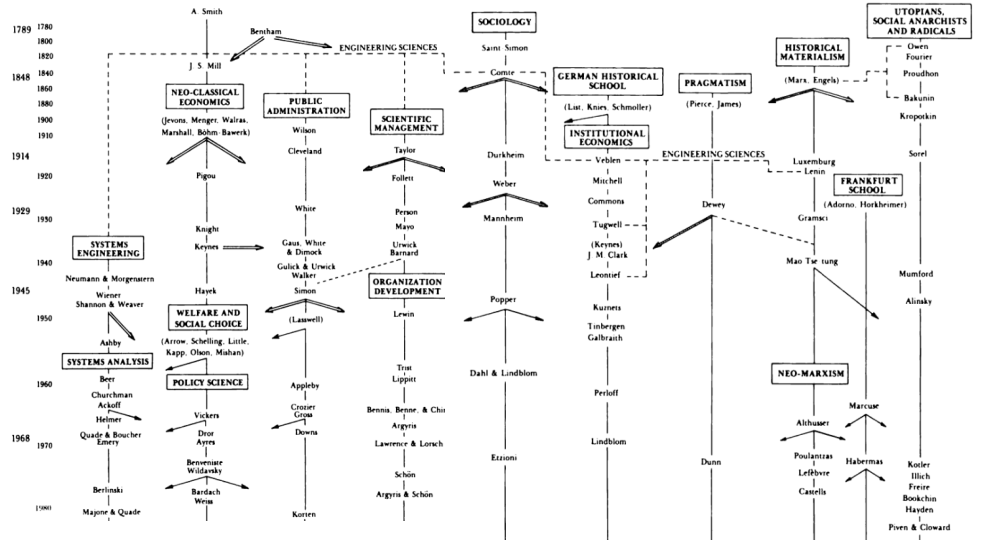
\includegraphics[scale=0.65]{Figures/chap2/friedman_timeline.png}
	\caption[Timeline of intellectual influences on American planning theory]{Timeline of intellectual influences on American planning theory. From \cite{mazza2017}}
	\label{fig:friedman_timeline}
\end{sidewaysfigure}
\clearpage

Also use diagram/framework from \cite{marcuseThreeHistoricCurrents2016}:

\begin{itemize}
    \setlength{\itemsep}{0pt}%
    \setlength{\parskip}{0pt}%
	\item{\textbf{Technicist:} Planning focused on maximizing efficient of the system being planned. The planner is a technical professional with specialized knowledge. The "technicist is inherently conservative: it is to serve an economic and social and policital order in which its role is to make that order function smoothly."}
	\item{\textbf{Social Reform:} Planning grounded in social ideas and values while viewing the necessary changes as possible within the exisiting framework of social, political, and economic order. The exact values of concern have varied over the years, with environmental sustainability coming to the rise more recently.}
	\item{\textbf{Social Justice:} Planning by grass-roots groups and social movements, putting values ahead of efficiency, and willing to work outside of existing systems to accomplish its goals.}
\end{itemize}


\begin{table}[h]
\caption[Axes of currents of city planning]{Axes of currents of city planning. Based on  \cite{marcuseThreeHistoricCurrents2016}}
\label{table:currents}
\begin{center}
\begin{tabular}{| C{0.1cm} C{0.1cm} | C{2cm} | C{3cm} | C{3cm} |} \cline{4-5}

\multicolumn{1}{c}{} & \multicolumn{1}{c}{} & \multicolumn{1}{c|}{} & \multicolumn{2}{c|}{\textit{Stance towards existing relations of power}}  \\ \cline{4-5}

\multicolumn{1}{c}{} & \multicolumn{1}{c}{} & \multicolumn{1}{c|}{} & \textbf{Critical} & \textbf{Deferential} \\ \hline

\multirow{4}{*}{\parbox{4cm}{\rotatebox[origin=c]{90}{\textit{Primary}}}}
& \multirow{4}{*}{\parbox{4cm}{\rotatebox[origin=c]{90}{\textit{concern}}}} 
& \multirow{2}{*}{\textbf{Social}} 
& \multirow{2}{*}{Social Justice} 
& \multirow{2}{*}{Social Reform} \\ 

& & & & \\ \cline{3-5}

& & \multirow{2}{*}{\textbf{Efficiency}} & & \multirow{2}{*}{Technicist} \\

& & & & \\  \hline

\end{tabular}
\end{center}
\end{table}



"The systems engineers bring some expertise and substantial pretensions to the problems of the city. Their prinicpal system expertise seems to be relative to complex organizations that are mission oriented. There is in any case a good deal of difference between the mission of reaching the moon, and the mission of surival and welfare for soceity and the city. The systems engineer can in general deal best with subsystems and specific tasks, and he therefore suboptimizes. This is a charitable description." \cite{robinsonDecisionmakingUrbanPlanning1972}

Goldman suggests that many of these issues can be avoided by paring complex systems theory with collaborative planning theory. \cite{goodspeedScenarioPlanningCities2020}

Goodman notes that "systems dynamics models are not widely used in urban practice" \cite{goodspeedScenarioPlanningCities2020}

Nostikasari notes how assumptions in a transportation planning model can perpetuate inequality \cite{nostikasariRepresentationsEverydayTravel2015}

"Are decision makers less likely to incorporate subjective values and humanistic concerns in policy decisions becaues of the seeming remoteness of hte world in which these policies have an impact?" \cite{vereginComputerInnovationAdoption1994}

This historic preference of the impersonal and "objective" versus the personal and "subjective" is by no means unique to systems engineering. It can also be found in economics, jurisprudence, education theory, political science, and even moral philosophy \cite{banuriModernatizationItsDiscontents1990}. The development of stakeholder analysis has helped to bridge the gap between these two and thus rectify this traditional deficiency. 

Participatory models were not unheard of even in earlier decades however. For example, the Dayton Neighborhod Achievement Model dates back to the early 1970s \cite{lightWarfareWelfareDefense2005}.

The use of stakeholder analysis in contemporary systems engineering is, in a way, a step away from the world view that sees "human beings as unknowable black boxes and machines as transparent," a viewpoint that "surrenders any attempt at empathy and forecloses the possibility of ethical development" and is a tacit "admission that we have abandoned a social commitment to try and understand each other." \cite{eubanksAutomatingInequalityHow2018}

Sufficient deficiencies certainly still remain within the systems engineering community. "One cannot know about the history of media stereotyping or the nuances of structural oppression in any formal, scholarly way through the traditional engineering curriculum of the large research universities from which technology companies hire across the United States. Ethics course are rare." \cite{nobleAlgorithmsOppressionHow2018}

It should be noted that, while \ac{ppgis} developed as a means to avoid some of these concerns, it also arose out of intra-academia discussion and arguments, not as a result of vociferous demand from communities themselves \cite{weinerParticipatoryGeographicInformation2007}. 

\subsection{Technocratic Planning and International Development} \label{sec:technocracy}

By "technocracy" we mean the basic idea that "the human problem of urban design has a unique solution, which an expert can discover and execute. Deciding such technical matters by politics and bargaining would lead to the wrong solution." \cite{scottSeeingStateHow2020}


Some of the sources here cited in this chapter refer specifically to maps, while others to more general quantified data for states. For our purposes, however, the differences between these two are not particularly important. Most "state simplications... have the character of maps. That is, they are designed to summarize precisely thoes aspects of a complex world that are of immediate interest to the mapmaker and to ignore the rest. To complain that a map lacks nuance and detail makes no sense unless it omits information necessary to its function." \cite{scottSeeingStateHow2020}


Respond to critiques of central planning / technocratic efforts by Easterly \cite{easterly2015}



James Scott argued that "legibility [is] a central problem in statecraft." Through the act of making society and nature itself legible, "officials took exceptionally, complex, illegible, and local social practices... and created a standard grid whereby it could be centrally recorded and monitored. The organization of hte natural world was no exception."  \cite{scottSeeingStateHow2020}


Scott argued that four elements were necessary to precipitate the most tragic of social engineering disasters \cite{scottSeeingStateHow2020}:

\begin{itemize} \setlength{\itemsep}{0pt} \setlength{\parskip}{0pt} 
	\item{The "administrative ordering of nature and society." This includes items like cadastral maps, surnames, census records, and a standardized legal system. As Theodore Porter put it, "Society must be remade before it can be the object of quantification." \cite{porter1992objectivity}}
	\item{A "high-modernist ideology," which Scott defines as a "strong," "muscle-bound" "self-confidence about scientific and technical progress, the expansion of production, the growing satisfaction of uman needs, the master of nature... and the rational design of social order commensurate with the scientific understanding of natural laws."}
	\item{An authoritarian state that is both "willing and able" to wield power to inact the high-modernist ideology.}
	\item{A vulnerable civil society that "lacks the capacity to resist" the plans of that authoritarian state.}
\end{itemize}

In essence what is "truly dangerous to us and our environment... is the \textit{combination} of the universalist pretensions of epistemic knowledge and authoritarian social engineering." \cite{scottSeeingStateHow2020}

With regard to the second element a key aspect is that, as Scott notes, high-modernist ideology is not scientific practice. It is a "faith that borrowed from the legitmacy of sciency and technology." In fact, it was more an aesthetic prediliction than anything scientific. Furthermore, the underlying ideas were in fact quite sympathetic. "Doctors and public-health engineers who did possess new knowledge that could save millions of lives were often thwarted by popular prejudices and entrenched political interests"  \cite{scottSeeingStateHow2020}. The dangers were when an authoritarian state adopted the aesthetic veilings of such ideas to justify actions, in the way that Social Darwinism used evolutionary theory to justify horrid actions. In this way "the classism and racism of elites are mathwashed, neutralized by technological mystification and data-based hocus-pocus." \cite{eubanksAutomatingInequalityHow2018} This ideology could also be considered a "dangerous form of magical thinking [that] often accompanies new technological developments, a curious assurance that a revolution in our tools inevitably wipes the slate of the past clean." \cite{eubanksAutomatingInequalityHow2018}


In the USSR, "a set of informal practices lying outside of the formal command economy - and often outside Soviet law as well - [arose] to circumvent some of the colossal waste and inefficiencies built into the system. Collectivized agriculture, in other words, never quite operated according to the hierarchical grid of production plans and procurements." \cite{scottSeeingStateHow2020} The technocratic leaders were often aware of this but so committed to their ideology that they had no alternative but to maintain a sort of pretense, which anthropologist Alexi Yurchak called 'hypernormalization' \cite{yurchakEverythingWasForever2005}, that served to compound problems until the Soviet Union eventually collapsed. Such a phenomena is particularly visible in strictly planned capital cities that have, "as the inevitable accompaniment of its official structures, given rise to another, far more 'disorderly' and complex city \textit{that makes the official city work} - that is virtually a condition of its existence." \cite{scottSeeingStateHow2020}



Even the successful development projects often came at a high cost and raised the question of "successful for whom?" After all "Haussmann's Paris was, \textit{for those who are not expelled}, a far healthier city." (emphasis mine) \cite{scottSeeingStateHow2020}


Facts generated by states are inherently simplifications. Specifically, they tend to simplify in five specific ways \cite{scottSeeingStateHow2020}:

\begin{itemize} \setlength{\itemsep}{0pt} \setlength{\parskip}{0pt} 
	\item{They are interested and utilitarian, aimed at a particular end.}
	\item{They are nearly always written, as opposed to visual or verbal.}
	\item{They are typically static and thus, perpetually out-of-date to at least some extent. "The cadastral map is very much like a still photograph of the current in a river."}
	\item{They are typically aggregate facts, not individual ones.}
	\item{They are standardized, so as to enable comparison and longitudinal analysis.}
\end{itemize}


Planning has come a long way from focusing on single page map and a timescale of 20-30 years (Section 2 Introduction of \cite{robinsonDecisionmakingUrbanPlanning1972})

By providing tools for more participation, we are not necessarily doing anything radical. "Democracies rarely end up expropriating and redistributing capital" \cite{fainsteinSpatialJusticePlanning2016}. "Participation is not power; its reform is not radical" \cite{marcuseThreeHistoricCurrents2016}. Some argue that neoliberalism in factor prefers to use participation as a means of underming resistance, rather than violence, though this has the risk of providing a structure for coalition building and radicalization \cite{miraftabInsurgentPlanningSituating2016}. In fact, increased community involvement can result in more restrictive, unambitious goals that are not in the interests of certain minorities (Section 1, Chapter 2 of \cite{robinsonDecisionmakingUrbanPlanning1972}).


Sachs argues that prescreptive economics should be modeled on clinical medicine and should not seek to attribute all negative outcomes to the same cause nor to prescribe the same solution to all problems, but instead to "make a differential diagnosis for the economic case at hand." He lays out several different conditions of poverty, for example, and proposes different solutions to each. Foreign aid is effective at treating the "poverty trap" condition (wherein "the country is too poor to make the basic investments it needs ot escape from extreme material deprivation and get on the ladder of economic growth"), but less so for other conditions.  \cite{sachsAgeSustainableDevelopment2015} We work with local collaborators to provide them with tools to develop local solutions....


Discuss and critique of informality as a concept \cite{royUrbanInformalityProduction2016}

De Soto argues that the poor already have assets, just needs to be formalized. \cite{sotoMysteryCapitalWhy2003} though others argue that this is just results in a cycle of appeasment / welfare \cite{hollandForbearanceRedistributionPolitics2017}

Power can be wielded in planning discussions in 
three primary ways: "by promoting formal decisions, setting the agenda, and influencing the broader ideogical context of the debate." (\cite{foresterPlanningFacePower2001} as paraphrased by \cite{goodspeedScenarioPlanningCities2020})

Goodspeed, however, argues that scenario-based planning can help address injustices such as racism in urban development and cites several examples of this having occured \cite{goodspeedScenarioPlanningCities2020}.

"Many studies involve ranking places on one or more criteria, and allocating policy benefits accordingly. At its crudest this applied geography merely provides a list of winner ans losers with no understanding of why the differences occur." \cite{taylorGeographicInformationSystems1994}

Part of this was sheer arrogance. Even one of the proponents recognized that "rational, hierarchical, closed-door decision strategies" had negative consequences and that "more democratic process might produces worse rsults, but it would respond to the increasing sense of alienation among the nation's urban population." \cite{lightWarfareWelfareDefense2005}

Virginia Eubanks proposees two gut check questions \cite{eubanksAutomatingInequalityHow2018}:

\begin{enumerate} \setlength{\itemsep}{0pt} \setlength{\parskip}{0pt} 
	\item{Does the tool increase the self-determinationa and agency of the poor?}
	\item{Would the tool be tolerated if it was targeted at non-poor people?}
\end{enumerate}

Jonathan Furner, meanwhile proposes three strategies (\cite{furner2007dewey} as paraphrased by \cite{nobleAlgorithmsOppressionHow2018}):

\begin{enumerate} \setlength{\itemsep}{0pt} \setlength{\parskip}{0pt} 
	\item{Admission on the part of designers that bias in classification schemes exists, and indeed is an inevitable result of the ways in which they are currently structured.}
	\item{Recognition that adherence to a policy of neutrality will contribute little to eradiction of htat bias and indeed can only extend its life.}
	\item{Construction, collection, and analysis of narrative expressions of the feelings, thoughts, and beliefs of classification-scheme users who identify with particularly racially-defined populations.}
\end{enumerate}



\begin{figure}[h]
	\centering
	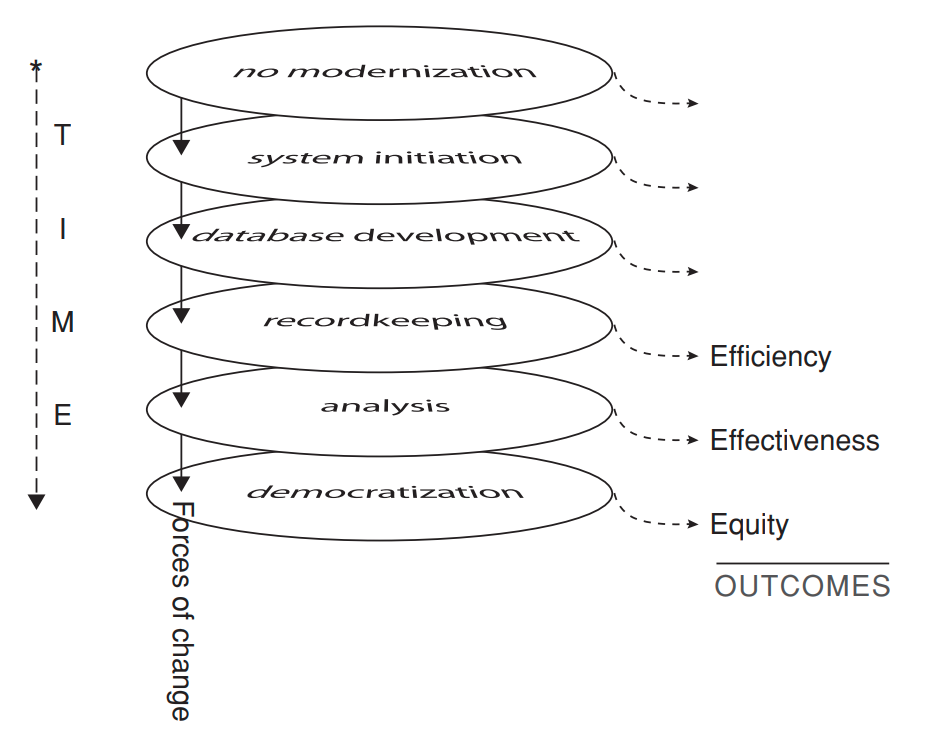
\includegraphics[scale=0.4]{Figures/chap2/gis_equity.png}
	\caption[Development of GIS development and associated outcomes]{Development of GIS development and associated outcomes. From \cite{tullochTheoreticalModelMultipurpose1999} as reprinted in \cite{tullochInstitutionalGeographicInformation2007}}
	\label{fig:gis_equity}
\end{figure}



\subsection{Sustainable Development and the SDGs}

"Substantive goals, the acievement of which are hard to measure, may be supplanted by thin, notional statistics - the number of villages formed, the number of acres plowed." \cite{scottSeeingStateHow2020}


"The pessimistic thought is that sustainable development has been stripped of its transformative power and reduced to its lowest common demoninator. After all, if both the World Bank and radical ecologists now believe in sustainability, the concept can have no teeth: it is so malleable as to mean many things to manny people without requiring commitment to any specific policies." \cite{campbellGreenCitiesGrowing2016}

"Yet there is also an optimistic interpretation of the broad empbrace given sustainability: the idea has become hegemonic, an accepted meta-narrative, a given. It has shifted from being a variable to being the parameter of hte debate, almost certain to be integrated into any future scenario of development." \cite{campbellGreenCitiesGrowing2016}

"To... critics, the prospect of integrating economic, environmental and equity interests will seem forced and artificial. States will require communities to prepare "Sustinable Development Master Plans," which will prove to be glib wish lists of goals and suspiciously vague implementation steps. To achieve consensus for the plan, language wil lbe reduced to the lowest common demoninator, and the pleasing plans will gather dust." (written in 1996, pre MDGs and SDGs) \cite{campbellGreenCitiesGrowing2016}

"The danger of translation is that one language will dominate the debate and thus define the terms of the solution. It is essential to exert equal effort to translate in each direction, to prevent one linguistic culture from dominating the other... Another lesson from the neocolonial inguistic experience is that it is crucial for each social group to express itself in its own language before any translation. The challenge for planners is to write the best translations among the languages of the economic, the ecological, and the social views, and to avoid a quasi-colonial dominance by the economic \textit{ingua franca}, by creating equal two-way translations... Translation can thus be a powerful planner's skill, and interdisciplinary planning education already provides some multiculturalism. Moreover, the idea of sustainability lends itself nicely to the meeting on common ground of competing value systems." \cite{campbellGreenCitiesGrowing2016}

Williamson and Connolly point out that "the term sustainability exists and operates within a number of governmental hegemonic discourses, i.e. the term itself is continually produced within legislative power structures," and argue that we should not "centre mapmaking praxis on generic or legislative definitions of sustainability, but rather encourages dialogue that supports the re-formation of self, community, and place." Importantly, they do not "seek to overturn generic understandings of sustainability, but rather seek a more complex understanding and proliferation of the term via local 'grounded' definitions. \cite{williamsonTheirworkDevelopmentSustainable2011} 


"That view is much too pessimistic... Investing in faireness may also be investing in efficiency, and... attention to sustainability can be more fair and more efficient at the same time." \cite{sachsAgeSustainableDevelopment2015}

"\ac{mdg} goal setting has energized civil society and helped to orient governments that otherwise might have neglected the chalenges of extreme poverty... the \acp{mdg} have been important in encouraging governments, experts, and civil society to undertake the 'differential diagnoses' necessary to overcome remaining obstacles." \cite{sachsAgeSustainableDevelopment2015}

Goals accomplish several things \cite{sachsAgeSustainableDevelopment2015}:

\begin{itemize}
    \setlength{\itemsep}{0pt}%
    \setlength{\parskip}{0pt}%
	\item{Global goals are critical for social mobilization and coordinated orientation.}
	\item{Global goals provide global peer pressure for adoption, monitoring, and action.}
	\item{Global goals mobilizing epistemic communities (experts, researchers, etc. These in turn can help map pathways to acheiving the goals, making them seem more managable and less remote.)}
	\item{Global goals mobilize stakeholder networks and thereby leverage capital and other resources.}
\end{itemize}

Even Sachs, a booster of global goals like the \acp{mdg} and \acp{sdg}, admitted that the impact of the \acp{mdg} was uneven, with public health receiving the most attention, while sanitation and education were largely sidelined. \cite{sachsAgeSustainableDevelopment2015}

\begin{figure}[h]
	\centering
	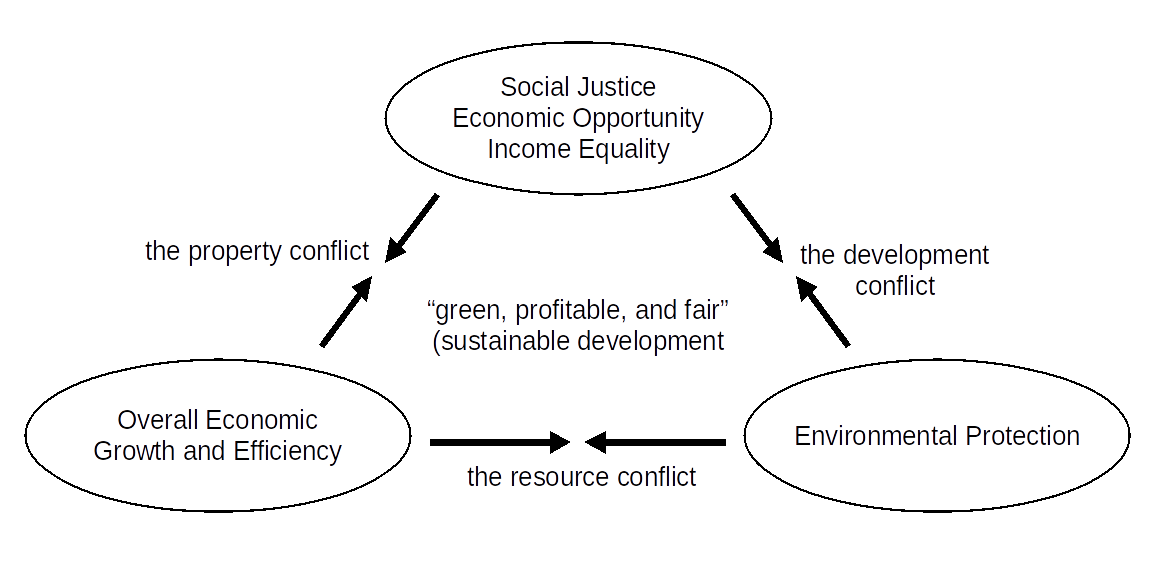
\includegraphics[scale=0.35]{Figures/chap2/sustainable_triangle.png}
	\caption[The triangle of conflicting goals of sustainable development]{The triangle of conflicting goals of sustainable development. Adapted from \cite{campbellGreenCitiesGrowing2016}}
	\label{fig:sustainable_triangle}
\end{figure}

Respond to critiques of \acp{mdg}/\acp{sdg} \cite{alstonShipsPassingNight2005, reddyGlobalDevelopmentGoals2008}



%\section{Section sample 1}


%\begin{enumerate}
%  \item Item 1.
%  \item Item 2.
%  \item Item 3.
%\end{enumerate}
%
%
%
%\begin{eqnarray*}
%a_i & = & a_j + a_k \\
%a_i & = & 2a_j + a_k \\
%a_i & = & 4a_j + a_k \\
%a_i & = & 8a_j + a_k \\
%a_i & = & a_j - a_k \\
%a_i & = & a_j \ll m \mbox{shift}
%\end{eqnarray*}
%instead of the multiplication.  For example, you could use:
%\begin{eqnarray*}
%r & = & 4s + s\\
%r & = & r + r
%\end{eqnarray*}
%Or by xx:
%\begin{eqnarray*}
%t & = & 2s + s \\
%r & = & 2t + s \\
%r & = & 8r + t
%\end{eqnarray*}
